\section{数据库设计概述}

\begin{itemize}
    \item 数据库设计是指对于一个给定的应用环境,构造(设计)优化的数据库逻辑模式和物理结构,并据此建立数据库及其应用系统,使之能够有效地存储和管理数据,满足各种用户的应用需求,包括信息管理要求和数据操作要求
    \begin{itemize}
        \item 信息管理要求:在数据库中应该存储和管理哪些数据对象
        \item 数据操作要求:对数据对象需要进行哪些操作,如查询、增、删、改、统计等操作
    \end{itemize}
    \item 数据库设计的目标是为用户和各种应用系统提供一个信息基础设施和高效率的运行环境
    \begin{itemize}
        \item 数据库数据的存取效率高
        \item 数据库存储空间的利用率高
        \item 数据库系统运行管理的效率高
    \end{itemize}
\end{itemize}

\subsection{数据库设计的特点}

\subsubsection{数据库建设的基本规律}
“三分技术,七分管理,十二分基础数据”
\begin{itemize}
    \item 管理
    \vspace{-0.8em}
	\begin{multicols}{2}
        \begin{itemize}
            \item 数据库建设项目管理 
            \item 企业(即应用部门)的业务管理
        \end{itemize}
	\end{multicols}
	\vspace{-1em}
    \item 基础数据
    \begin{itemize}
        \item 数据的收集、整理、组织和不断更新
    \end{itemize}
\end{itemize}

\subsubsection{结构(数据)设计和行为(处理)设计相结合}
\begin{itemize}
    \item 将数据库结构设计和数据处理设计密切结合
    \item 结构和行为分离的设计
    \begin{itemize}
        \item 传统的软件工程:重行为设计,忽视对应用中数据语义的分析和抽象,只要有可能就尽量推迟数据结构设计的决策
        \item 早期的数据库设计:重结构设计,致力于数据模型和数据库建模方法研究,忽视了行为设计对结构设计的影响
    \end{itemize}
\end{itemize}

\subsection{数据库设计方法}
\begin{itemize}
    \item 大型数据库设计是涉及多学科的综合性技术,又是一项庞大的工程项目。
    \item 它要求多方面的知识和技术。主要包括:
    \vspace{-0.8em}
	\begin{multicols}{3}
        \begin{itemize}
            \item 计算机的基础知识
            \item 软件工程的原理和方法
            \item 程序设计的方法和技巧
            \item 数据库的基本知识
            \item 数据库设计技术
            \item 应用领域的知识
        \end{itemize}
	\end{multicols}
	\vspace{-1em}
    \item 手工试凑法
    \item 规范设计法
    \vspace{-0.8em}
	\begin{multicols}{2}
        \begin{itemize}
            \item 新奥尔良(New Orleans)方法
            \item 基于 E-R 模型的数据库设计方法
            \item 3NF(第三范式)的设计方法
            \item 面向对象的数据库设计方法
            \item 统一建模语言(UML)方法
        \end{itemize}
	\end{multicols}
	\vspace{-1em}
\end{itemize}

\subsection{数据库设计的基本步骤}
\begin{figure}[H]
    \vspace{-0.5em}
	\centering
	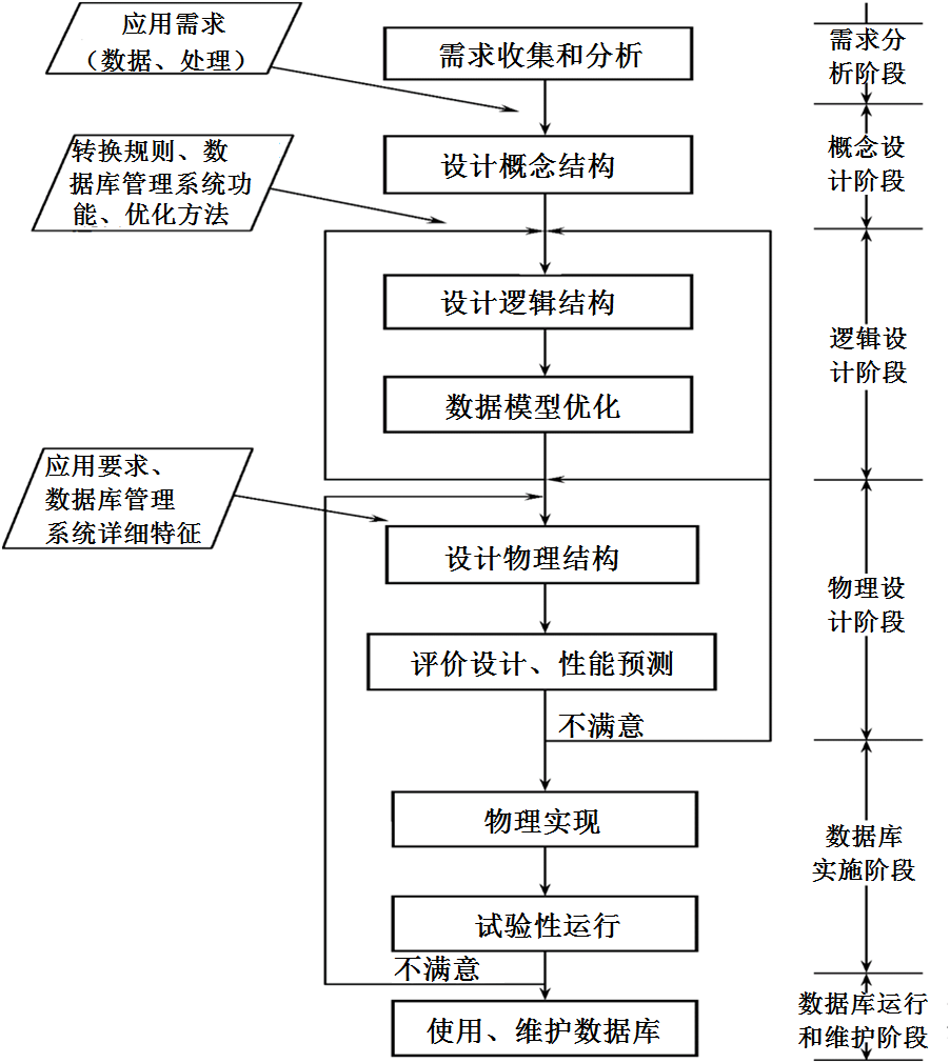
\includegraphics[width=0.5\textwidth]{images/7.1.3}
    \vspace{-1em}
\end{figure}

数据库设计各个阶段的数据设计描述
\begin{figure}[H]
    \vspace{-0.5em}
	\centering
	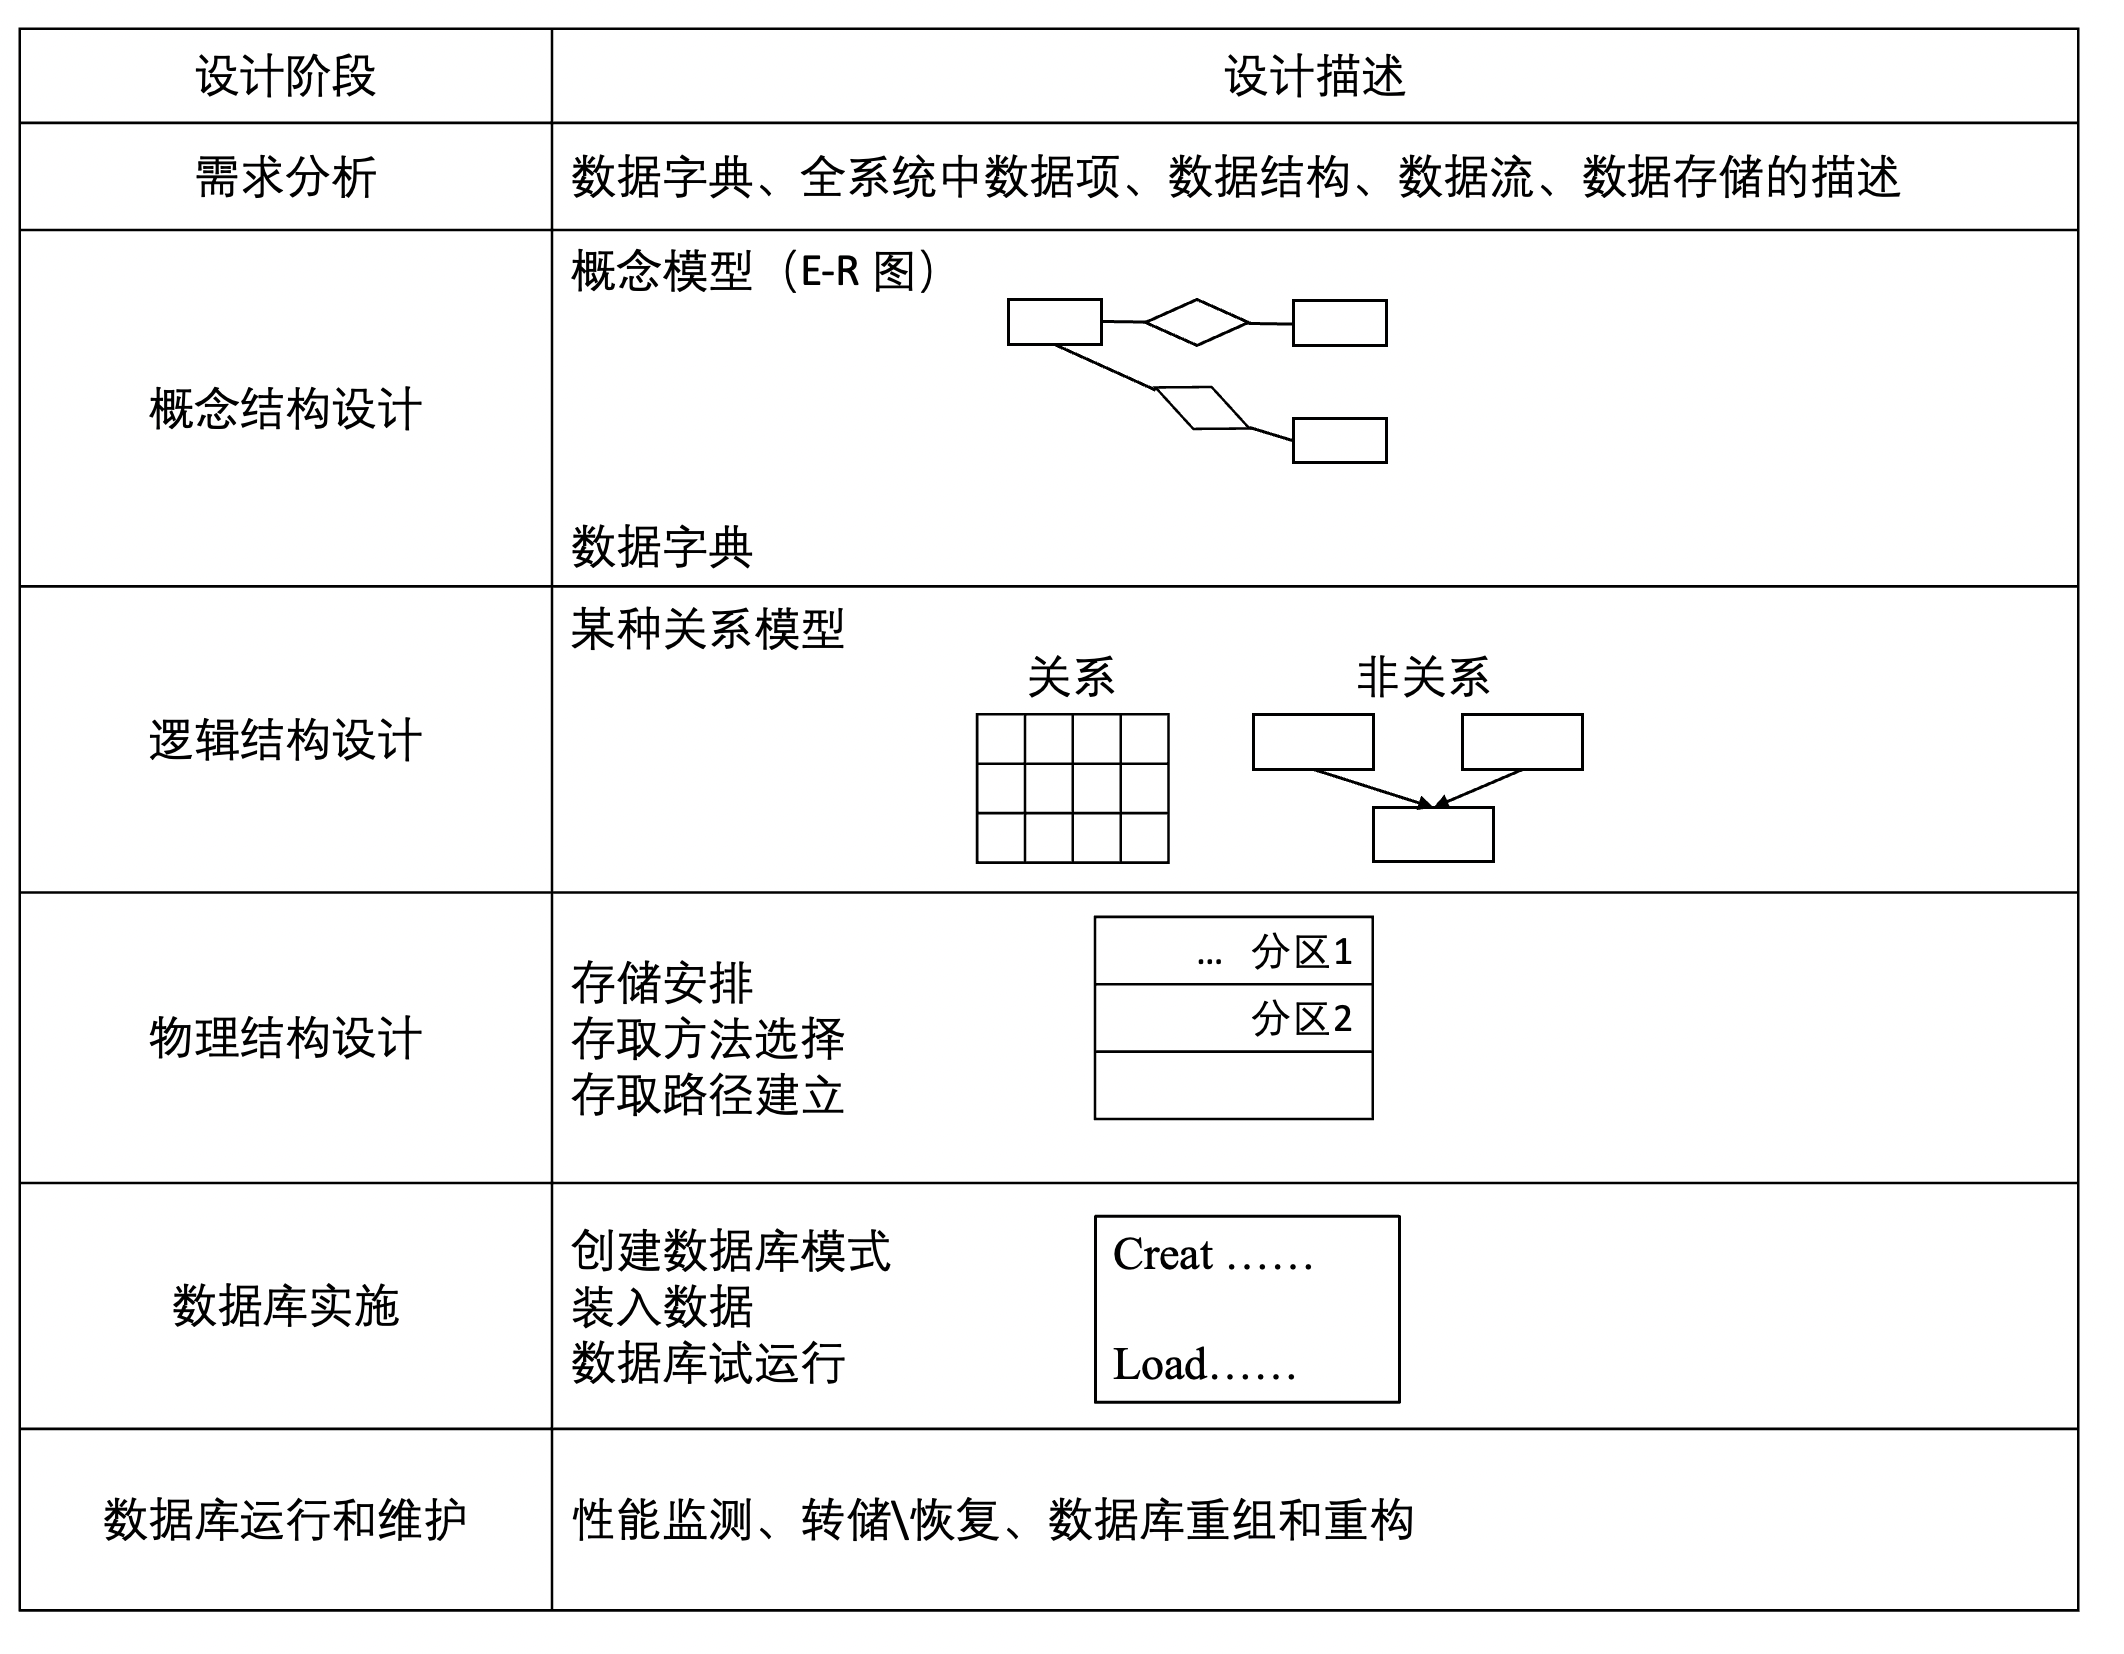
\includegraphics[width=0.6\textwidth]{images/7.1.3.2}
    \vspace{-1em}
\end{figure}

\subsection{数据库设计过程中的各级模式}
\begin{figure}[H]
    \vspace{-0.5em}
	\centering
	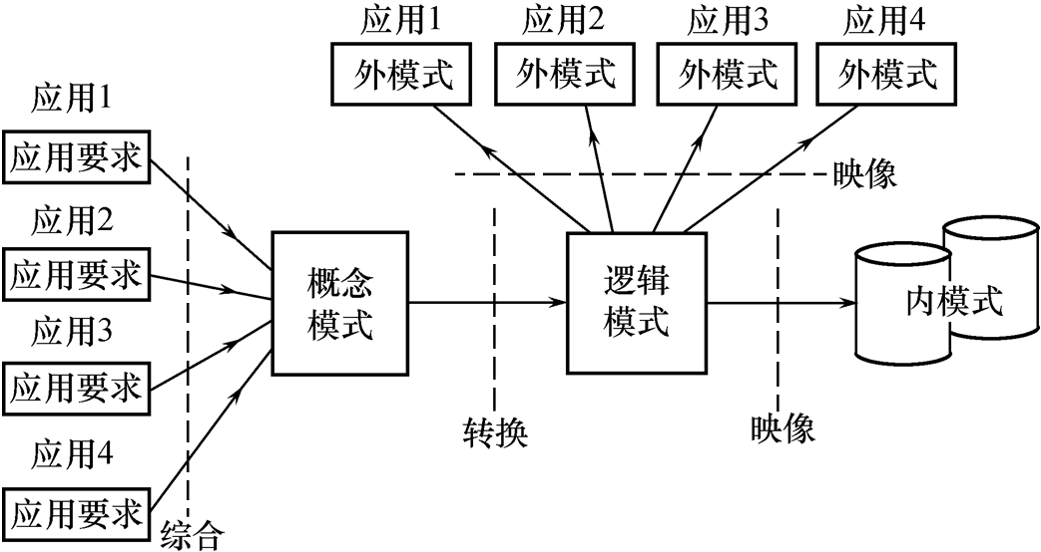
\includegraphics[width=0.5\textwidth]{images/7.1.4}
    \vspace{-1em}
\end{figure}

\section{需求分析}

\subsection{需求分析的任务}
\begin{itemize}
    \item 详细调查现实世界要处理的对象(组织、部门、企业等)
    \item 充分了解原系统(手工系统或计算机系统)工作概况
    \item 明确用户的各种需求
    \item 在此基础上确定新系统的功能
    \item 新系统必须充分考虑今后可能的扩充和改变
    \item 调查的重点是“数据”和“处理”,获得用户对数据库的要求
    \begin{itemize}
        \item 信息要求
        \begin{itemize}
            \item 用户需要从数据库中获得信息的内容与性质
            \item 由信息要求可以导出数据要求,即在数据库中需要存储哪些数据
        \end{itemize}
        \item 处理要求
        \begin{itemize}
            \item 用户要完成的处理功能
            \item 对处理性能的要求
        \end{itemize}
        \item 安全性与完整性要求
    \end{itemize}
    \item 确定用户最终需求的难点
    \begin{itemize}
        \item 用户缺少计算机知识,不能准确地表达自己的需求,他们所提出的需求往往不断地变化
        \item 设计人员缺少用户的专业知识,不易理解用户的真正需求,甚至误解用户的需求
    \end{itemize}
    \item 解决方法
    \item 设计人员必须不断深入地与用户进行交流,才能逐步确定用户的实际需求  
\end{itemize}

\subsection{需求分析的方法}
\begin{enumerate}[label=\arabic*.]
    \item 调查组织机构情况
    \item 调查各部门的业务活动情况
    \item 协助用户明确对新系统的各种要求,包括信息要求、处理要求、完全性与完整性要求
    \item 确定新系统的边界
\end{enumerate}
\begin{figure}[H]
    \vspace{-0.5em}
	\centering
	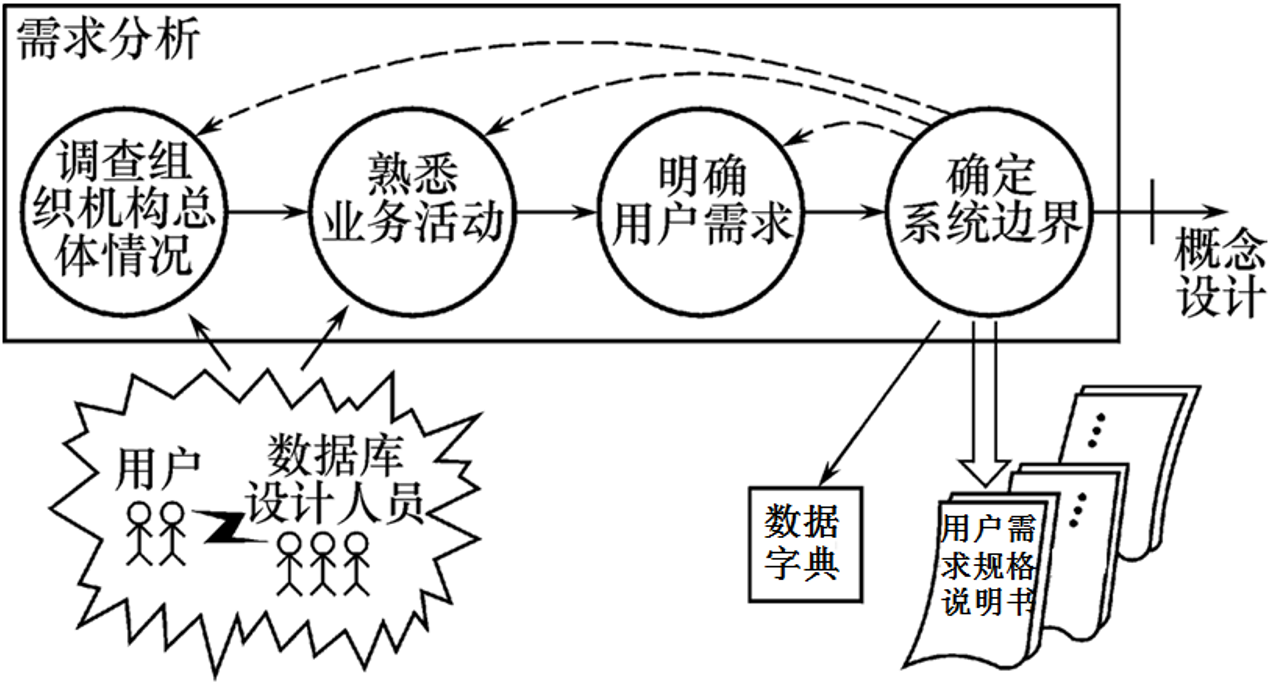
\includegraphics[width=0.5\textwidth]{images/7.2.2}
    \vspace{-1em}
\end{figure}

\subsection{数据字典}
\begin{itemize}
    \item 数据字典是关于数据库中数据的描述,即元数据,不是数据本身
    \item 数据字典在需求分析阶段建立,在数据库设计过程中不断修改、充实、完善
    \item 数据字典是进行详细的数据收集和数据分析所获得的主要结果 
    \item 数据字典的内容
    \vspace{-0.8em}
	\begin{multicols}{3}
        \begin{itemize}
            \item 数据项
            \item 数据结构
            \item 数据流
            \item 数据存储
            \item 处理过程
        \end{itemize}
	\end{multicols}
	\vspace{-1em}
    \item 数据项是数据的最小组成单位
    \item 若干个数据项可以组成一个数据结构
    \item 数据字典通过对数据项和数据结构的定义来描述数据流、数据存储的逻辑内容
\end{itemize}

\subsubsection{数据项}
\begin{itemize}
    \item 数据项是不可再分的数据单位
    \item 对数据项的描述:数据项描述$=$\{数据项名,数据项含义说明,别名,数据类型,长度,取值范围,取值含义,与其他数据项的逻辑关系,数据项之间的联系\}
    \begin{itemize}
        \item “取值范围”、“与其他数据项的逻辑关系”定义了数据的完整性约束条件,是设计数据检验功能的依据
        \item 可以用关系规范化理论为指导,用数据依赖的概念分析和表示数据项之间的联系
    \end{itemize}
\end{itemize}

\subsubsection{数据结构}
\begin{itemize}
    \item 数据结构反映了数据之间的组合关系。
    \item 一个数据结构可以由若干个数据项组成,也可以由若干个数据结构组成,或由若干个数据项和数据结构混合组成
    \item 对数据结构的描述:数据结构描述$=$\{数据结构名,含义说明,组成:\{数据项或数据结构\}\}
\end{itemize}

\subsubsection{数据流}
\begin{itemize}
    \item 数据流是数据结构在系统内传输的路径
    \item 对数据流的描述:数据流描述$=$\{数据流名,说明,数据流来源,数据流去向,组成:\{数据结构\},平均流量,高峰期流量\}
    \begin{itemize}
        \item 数据流来源:说明该数据流来自哪个过程
        \item 数据流去向:说明该数据流将到哪个过程去
        \item 平均流量:在单位时间(每天、每周、每月等)里的传输次数
        \item 高峰期流量:在高峰时期的数据流量
    \end{itemize}
\end{itemize}

\subsubsection{数据存储}
\begin{itemize}
    \item 数据存储是数据结构停留或保存的地方,也是数据流的来源和去向之一。
    \item 对数据存储的描述:数据存储描述$=$\{数据存储名,说明,编号,输入的数据流,输出的数据流,组成:\{数据结构\},数据量,存取频度,存取方式\}
    \begin{itemize}
        \item 存取频度:每小时、每天或每周存取次数,每次存取的数据量等信息 
        \item 存取方法:批处理/联机处理;检索/更新;顺序检索/随机检索
        \item 输入的数据流:数据来源
        \item 输出的数据流:数据去向
    \end{itemize}
\end{itemize}

\subsubsection{处理过程}
\begin{itemize}
    \item 处理过程的具体处理逻辑一般用判定表或判定树来描述。数据字典中只需要描述处理过程的说明性信息
    \item 处理过程说明性信息的描述:处理过程描述$=$\{处理过程名,说明,输入:\{数据流\},输出:\{数据流\},处理:\{简要说明\}\}
    \begin{itemize}
        \item 简要说明:说明该处理过程的功能及处理要求
        \begin{itemize}
            \item 功能:该处理过程用来做什么
            \item 处理要求:处理频度要求,如单位时间里处理多少事务,多少数据量、响应时间要求等
            \item 处理要求是后面物理设计的输入及性能评价的标准
        \end{itemize}
    \end{itemize}
\end{itemize}

\section{概念结构设计}

\subsection{概念模型}
\begin{itemize}
    \item 将需求分析得到的用户需求抽象为信息结构(即概念模型)的过程就是概念结构设计
    \item 概念模型的特点:
    \begin{itemize}
        \item 能真实、充分地反映现实世界,是现实世界的一个真实模型
        \item 易于理解,从而可以用它和不熟悉计算机的用户交换意见
        \item 易于更改,当应用环境和应用要求改变时,容易对概念模型修改和扩充
        \item 易于向关系、网状、层次等各种数据模型转换
    \end{itemize}
    \item 描述概念模型的工具:E-R模型
\end{itemize}

\subsection{E-R模型}

\subsubsection{实体之间的联系}

\paragraph*{两个实体型之间的联系}~{}
\begin{itemize}
    \item 一对一联系($1:1$):如果对于实体集 A 中的每一个实体,实体集 B 中至多有一个(也可以没有)实体与之联系,反之亦然,则称实体集 A 与实体集 B 具有一对一联系,记为$1:1$
    \item 一对多联系($1:n$):如果对于实体集 A 中的每一个实体,实体集 B 中有 $n$ 个实体($n\geq 0$)与之联系,反之,对于实体集 B 中的每一个实体,实体集 A 中至多只有一个实体与之联系,则称实体集 A 与实体集 B 有一对多联系,记为$1:n$ 
    \item 多对多联系($m:n$):如果对于实体集 A 中的每一个实体,实体集 B 中有 $n$ 个实体($n\geq 0$)与之联系,反之,对于实体集 B 中的每一个实体,实体集 A 中也有 $m$ 个实体($m\geq 0$)与之联系,则称实体集 A 与实体集 B 具有多对多联系,记为$m:n$
\end{itemize}

\begin{figure}[H]
    \vspace{-0.5em}
	\centering
	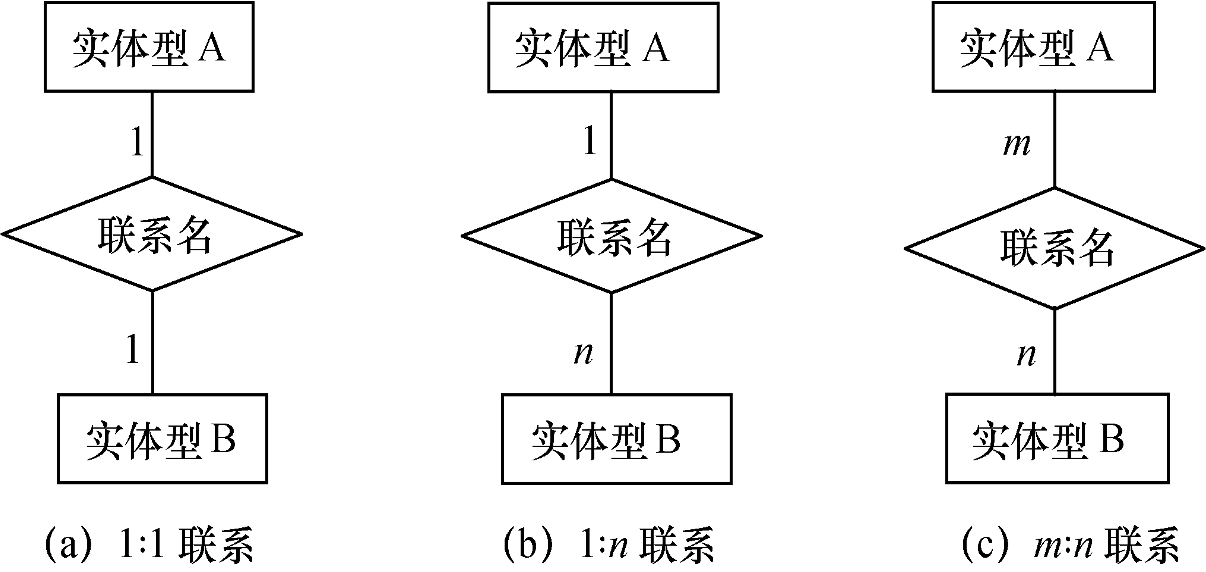
\includegraphics[width=0.5\textwidth]{images/7.3.2.1.1}
    \vspace{-1em}
\end{figure}

\paragraph*{两个以上的实体型之间的联系}~{}

两个以上的实体型之间也存在着一对一、一对多、多对多联系
\begin{figure}[H]
    \vspace{-0.5em}
	\centering
	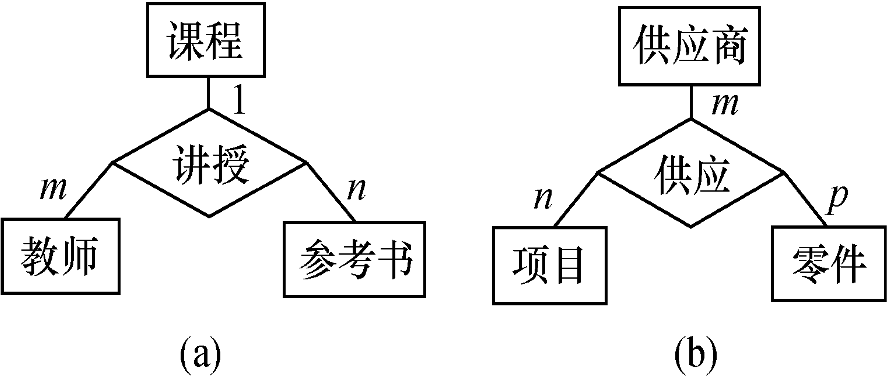
\includegraphics[width=0.45\textwidth]{images/7.3.2.1.2}
    \vspace{-1em}
\end{figure}

\paragraph*{单个实体型内的联系}~{}

同一个实体集内的各实体之间也可以存在一对一、一对多、多对多的联系
\begin{figure}[H]
    \vspace{-0.5em}
	\centering
	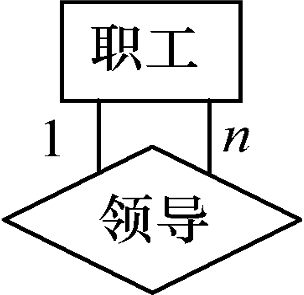
\includegraphics[width=0.13\textwidth]{images/7.3.2.1.3}
    \vspace{-1em}
\end{figure}

\subsubsection{E-R图}
E-R图提供了表示实体型、属性和联系的方法:
\begin{itemize}
    \item 实体型:用矩形表示,矩形框内写明实体名
    \item 属性:用椭圆形表示,并用无向边将其与相应的实体型连接起来
    \item 联系:用菱形表示,菱形框内写明联系名,并用无向边分别与有关实体型连接起来,同时在无向边旁标上联系的类型($1:1$、$1:n$ 或 $m:n$)
    \item 联系可以具有属性
\end{itemize}

\subsection{拓展的E-R模型}

\subsubsection{ISA联系}
\begin{itemize}
    \item 有的实体型是某个实体型的子类型,这种父类—子类联系称为 ISA 联系,表示“is a”语义。用$\triangle$表示
    \item ISA联系的性质: 子类继承了父类的所有属性,子类也可以有自己的属性
\end{itemize}

\paragraph*{分类属性}~{}

\begin{itemize}
    \item 分类属性是父实体型的一个属性
    \item 分类属性的值把父实体型中的实体分派到子实体型中 
\end{itemize}

\begin{figure}[H]
    \vspace{-0.5em}
	\centering
	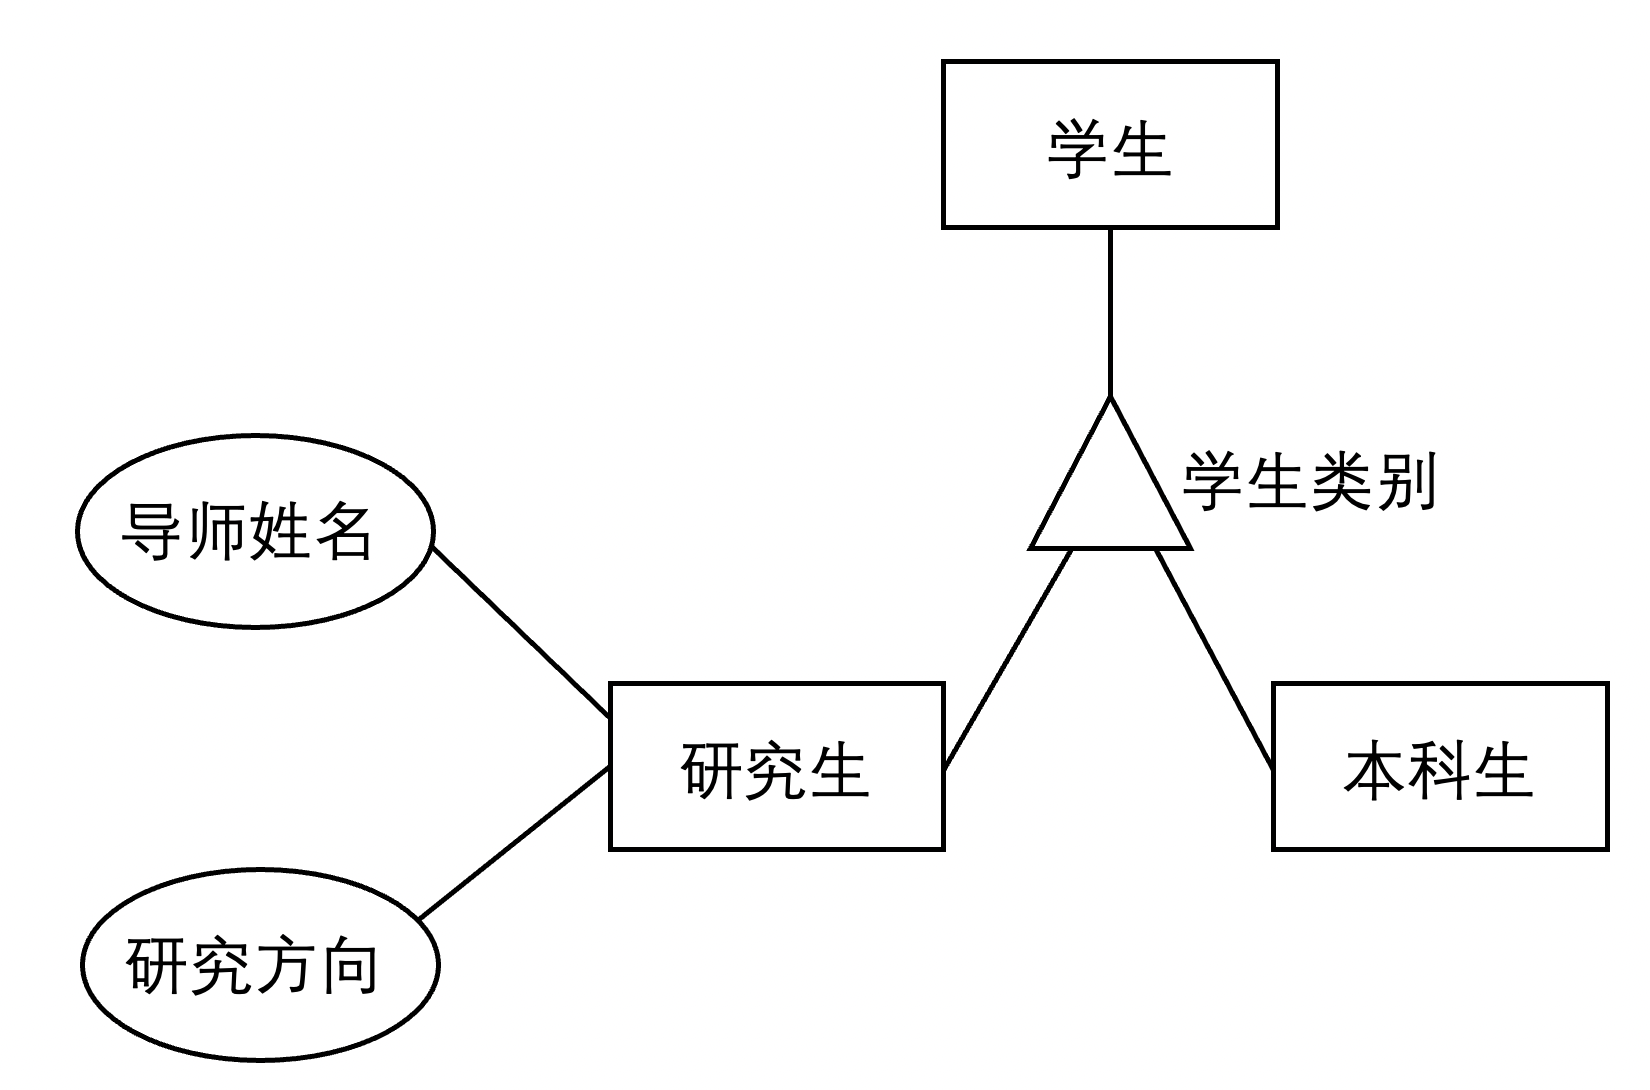
\includegraphics[width=0.45\textwidth]{images/7.12}
    \vspace{-1em}
\end{figure}

\paragraph*{不相交约束与可重叠约束}~{}

\begin{itemize}
    \item 不相交约束:描述父类中的一个实体不能同时属于多个子类中的实体集。即一个父类中的实体最多属于一个子类实体集
    \item 用 ISA 联系符号三角形内加一个叉号“$\times$"来表示
    \item 可重叠约束:父类中的一个实体能同时属于多个子类中的实体集。子类符号中没有叉号表示是可重叠的
\end{itemize}

\begin{figure}[H]
    \vspace{-0.5em}
	\centering
	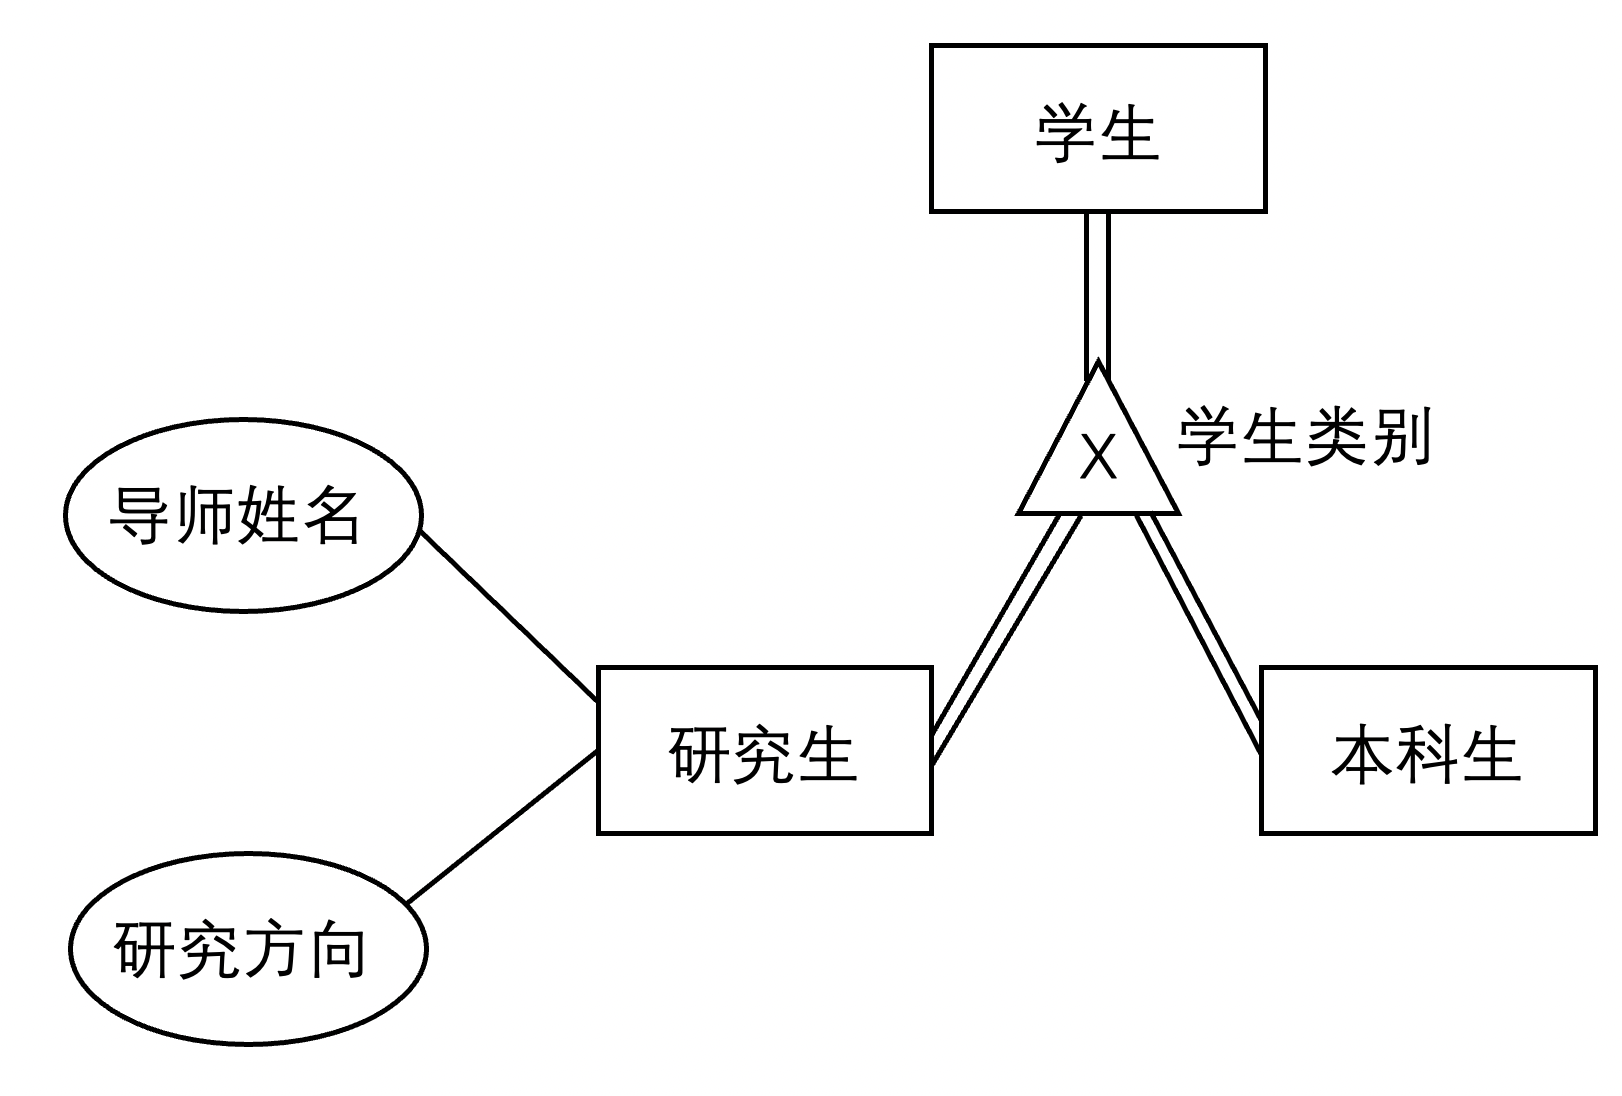
\includegraphics[width=0.45\textwidth]{images/7.13}
    \vspace{-1em}
\end{figure}

\paragraph*{完备性约束}~{}

\begin{itemize}
    \item 描述父类中的一个实体是否必须是某一个子类中的实体
    \begin{itemize}
        \item 如果是,则叫做完全特化(total specialization)
        \item 否则叫做部分特化(partial specialization)
    \end{itemize}
    \item 完全特化用父类到子类的双线连接来表示
    \item 部分特化用父类到子类的单线连接来表示
\end{itemize}

\subsubsection{基数约束}
\begin{itemize}
    \item 说明实体型中的任何一个实体可以在联系中出现的最少次数和最多次数
    \item 对实体之间一对一、 一对多、多对多联系的细化
    \item 约束用一个数对 $\min .. \max$ 表示,$0\leq \min \leq \max$。例如 $0..1,1..3,1..*$,其中 $*$ 代表无穷大
    \item $\min=1$ 的约束叫做强制参与约束,即被施加基数约束的实体型中的每个实体都要参与联系
    \item $\min=0$ 的约束叫做非强制参与约束,被施加基数约束的实体型中的实体可以出现在联系中,也可以不出现在联系
\end{itemize}

\subsubsection{Part-of联系}
\begin{itemize}
    \item 描述某个实体型是另外一个实体型的一部分
    \item Part-of 联系可以分为两种情况:
    \begin{itemize}
        \item 非独占的 Part-of 联系,简称非独占联系
        \begin{itemize}
            \item 整体实体如果被破坏,另一部分实体仍然可以独立存在
        \end{itemize}
        \item 独占的 Part-of联系,简称独占联系
        \begin{itemize}
            \item 整体实体如果被破坏,部分实体不能存在
        \end{itemize}
    \end{itemize}
    \item Part-of 联系的表示
    \begin{itemize}
        \item 用非强制参与联系表示非独占的 Part-of 联系
        \item 用弱实体类型和识别联系来表示独占联系编号
    \end{itemize}
    \item 如果一个实体型的存在依赖于其它实体型的存在,则这个实体型叫做弱实体型,否则叫做强实体型
    \item 用弱实体类型和识别联系来表示独占联系双矩形表示弱实体型,用双菱型表示识别联系
\end{itemize}

\subsection{概念结构设计}

\subsubsection{实体与属性的划分原则}
\begin{itemize}
    \item 作为属性,不能再具有需要描述的性质。属性必须是不可分的数据项,不能包含其他属性
    \item 属性不能与其他实体具有联系,即E-R图中所表示的联系是实体之间的联系
\end{itemize}

\subsubsection{E-R图的集成}
E-R 图的集成一般需要分两步
\begin{itemize}
    \item 合并。解决各分 E-R 图之间的冲突,将分 E-R 图合并起来生成初步 E-R 图
    \item 修改和重构。消除不必要的冗余,生成基本 E-R 图
\end{itemize}

\paragraph*{合并E-R图,生成初步E-R图}~{}

各个局部应用所面向的问题不同,各个子系统的 E-R 图之间必定会存在许多不一致的地方,称之为冲突

子系统 E-R 图之间的冲突主要有三类:
\begin{itemize}
    \item 属性冲突
    \begin{itemize}
        \item 属性域冲突,即属性值的类型、取值范围或取值集合不同
        \item 属性取值单位冲突
    \end{itemize}
    \item 命名冲突
    \begin{itemize}
        \item 同名异义,即不同意义的对象在不同的局部应用中具有相同的名字
        \item 异名同义(一义多名),即同一意义的对象在不同的局部应用中具有不同的名字    
    \end{itemize}
    \item 结构冲突
    \begin{itemize}
        \item 同一对象在不同应用中具有不同的抽象
        \begin{itemize}
            \item 解决方法:把属性变换为实体或把实体变换为属性,使同一对象具有相同的抽象。但仍然要遵循实体与属性的划分原则
        \end{itemize}
        \item 同一实体在不同子系统的 E-R 图中所包含的属性个数和属性排列次序不完全相同
        \begin{itemize}
            \item 解决方法:使该实体的属性取各子系统的 E-R 图中属性的并集,再适当调整属性的次序
        \end{itemize}
        \item 实体间的联系在不同的 E-R 图中为不同的类型
    \end{itemize}
\end{itemize}

\paragraph*{消除不必要的冗余,设计基本E-R图}~{}

\begin{itemize}
    \item 所谓冗余的数据是指可由基本数据导出的数据,冗余的联系是指可由其他联系导出的联系
    \item 消除冗余主要采用分析方法,即以数据字典和数据流图为依据,根据数据字典中关于数据项之间逻辑关系的说明来消除冗余
\end{itemize}

\section{逻辑结构设计}

\subsection{E-R图向关系模型的转换}
\begin{itemize}
    \item 一个 $1:1$ 联系可以转换为一个独立的关系模式,也可以与任意一端对应的关系模式合并
    \item 一个 $1:n$ 联系可以转换为一个独立的关系模式,也可以与 $n$ 端对应的关系模式合并
    \item 一个 $m:n$ 联系转换为一个关系模式,与该联系相连的各实体部分的码以及联系本身的属性均转换为关系的属性,各实体的码组成关系的码或关系码的一部分
    \item 三个或三个以上实体间的一个多元联系转换为一个关系模式
    \item 具有相同码的关系模式可合并
\end{itemize}

\subsection{数据模型的优化}
关系数据模型的优化通常以规范化理论为指导,方法为:
\begin{itemize}
    \item 确定数据依赖
    \item 对于各个关系模式之间的数据依赖进行极小化处理,消除冗余的联系
    \item 按照数据依赖的理论对关系模式进行分析,考察是否存在部分函数依赖、传递函数依赖、多值依赖等,确定各关系模式分别属于第几范式
    \item 按照需求分析阶段得到的各种应用对数据处理的要求,分析对于这样的应用环境这些模式是否合适,确定是否要对它们进行合并或分解
    \item 对关系模式进行必要分解,提高数据操作效率和存储空间的利用率
\end{itemize}

\subsection{设计用户子模式}
\begin{itemize}
    \item 定义数据库模式主要是从系统的时间效率、空间效率、易维护等角度出发
    \item 定义用户外模式时应该更注重考虑用户的习惯与方便。包括三个方面:
    \begin{itemize}
        \item 使用更符合用户习惯的别名
        \begin{itemize}
            \item 合并各分 E-R 图曾做了消除命名冲突的工作,以使数据库系统中同一关系和属性具有唯一的名字。这在设计数据库整体结构时是非常必要的
            \item 用视图机制可以在设计用户视图时可以重新定义某些属性名,使其与用户习惯一致,以方便使用
        \end{itemize}
        \item 针对不同级别的用户定义不同的视图,以保证系统的安全性
        \item 简化用户对系统的使用
        \begin{itemize}
            \item 如果某些局部应用中经常要使用某些很复杂的查询,为了方便用户,可以将这些复杂查询定义为视图
        \end{itemize}
    \end{itemize}
\end{itemize}

\section{数据库的物理设计}
\begin{itemize}
    \item 数据库在物理设备上的存储结构与存取方法称为数据库的物理结构,它依赖于选定的数据库管理系统
    \item 为一个给定的逻辑数据模型选取一个最适合应用要求的物理结构的过程,就是数据库的物理设计
    \item 数据库物理设计的步骤
    \begin{itemize}
        \item 确定数据库的物理结构,在关系数据库中主要指存取方法和存储结构
        \item 对物理结构进行评价,评价的重点是时间和空间效率   
    \end{itemize}
    \item 若评价结果满足原设计要求,则可进入到物理实施阶段。否则,就需要重新设计或修改物理结构,有时甚至要返回逻辑设计阶段修改数据模型
\end{itemize}

\subsection{数据库物理设计的内容和方法}
\begin{itemize}
    \item 设计物理数据库结构的准备工作
    \begin{itemize}
        \item 充分了解应用环境,详细分析要运行的事务,以获得选择物理数据库设计所需参数
        \item 充分了解所用关系型数据库管理系统的内部特征,特别是系统提供的存取方法和存储结构
    \end{itemize}
    \item 关系数据库物理设计的内容
    \begin{itemize}
        \item 为关系模式选择存取方法
        \item 设计关系、索引等数据库文件的物理存储结构
    \end{itemize}
    \item 物理数据库设计所需参数
    \begin{itemize}
        \item 数据库查询事务
        \vspace{-0.8em}
        \begin{multicols}{2}
            \begin{itemize}
                \item 查询的关系
                \item 查询条件所涉及的属性
                \item 连接条件所涉及的属性
                \item 查询的投影属性
            \end{itemize}
        \end{multicols}
        \vspace{-1em}
        \item 数据更新事务
        \begin{itemize}
            \item 被更新的关系
            \item 每个关系上的更新操作条件所涉及的属性
            \item 修改操作要改变的属性值
        \end{itemize}
        \item 每个事务在各关系上运行的频率和性能要求
    \end{itemize}
\end{itemize}

\subsection{关系模式存取方法选择}
\begin{itemize}
    \item 数据库系统是多用户共享的系统,对同一个关系要建立多条存取路径才能满足多用户的多种应用要求
    \item 物理结构设计的任务之一是根据关系数据库管理系统支持的存取方法确定选择哪些存取方法
    \item 数据库管理系统常用存取方法
    \vspace{-0.8em}
    \begin{multicols}{3}
        \begin{itemize}
            \item B+ 树索引存取方法
            \item Hash 索引存取方法
            \item 聚簇存取方法
        \end{itemize}
    \end{multicols}
    \vspace{-1em}
\end{itemize}

\subsubsection{B+树索引存取方法的选择}
\begin{itemize}
    \item 选择索引存取方法的主要内容:根据应用要求确定对哪些属性列建立索引、对哪些属性列建立组合索引、对哪些索引要设计为唯一索引
    \item 选择索引存取方法的一般规则
    \begin{itemize}
        \item 如果一个(或一组)属性经常在查询条件中出现,则考虑在这个(或这组)属性上建立索引(或组合索引)
        \item 如果一个属性经常作为最大值和最小值等聚集函数的参数,则考虑在这个属性上建立索引
        \item 如果一个(或一组)属性经常在连接操作的连接条件中出现,则考虑在这个(或这组)属性上建立索引
    \end{itemize}
    \item 关系上定义的索引数过多会带来较多的额外开销(维护、查找索引的开销)
\end{itemize}

\subsubsection{Hash索引存取方法的选择}
选择 Hash 存取方法的规则
\begin{itemize}
    \item 如果一个关系的属性主要出现在等值连接条件中或主要出现在等值比较选择条件中,而且满足下列两个条件之一
    \begin{itemize}
        \item 该关系的大小可预知,而且不变
        \item 该关系的大小动态改变,但所选用的数据库管理系统提供了动态 Hash 存取方法
    \end{itemize}
\end{itemize}

\subsubsection{聚簇存取方法的选择}
\begin{itemize}
    \item 为了提高某个属性(或属性组)的查询速度,把这个或这些属性(称为聚簇码)上具有相同值的元组集中存放在连续的物理块中称为聚簇
    \item 该属性(或属性组)称为聚簇码(cluster key)
    \item 聚簇的用途:大大提高按聚簇属性进行查询的效率  
    \item 聚簇既适用于单个关系,也适用于经常进行连接操作的多个关系
    \begin{itemize}
        \item 把多个连接的元组按连接属性值聚集存放
        \item 从而实现多个关系的“预连接”,提高连接操作的效率
    \end{itemize} 
\end{itemize}

聚簇存储方法的选择
\begin{itemize}
    \item 选择聚簇存储方法,即确定需要建立多少个聚簇,每个聚簇中包含哪些关系(一个数据库可以建立多个聚簇,一个关系只能加入一个聚簇)
    \item 设计候选聚簇
    \begin{itemize}
        \item 常在一起进行连接操作的关系可以建立组合聚簇
        \item 如果一个关系的一组属性经常出现在相等比较条件中,则该单个关系可建立聚簇
        \item 如果一个关系的一个(或一组)属性上的值重复率很高,则此单个关系可建立聚簇
    \end{itemize}
    \item 检查候选聚簇中的关系,取消其中不必要的关系
    \begin{itemize}
        \item 从聚簇中删除经常进行全表扫描的关系
        \item 从聚簇中删除更新操作远多于连接操作的关系
        \item 从聚簇中删除重复出现的关系
        \begin{itemize}
            \item 当一个关系同时加入多个聚簇时,必须从这多个聚簇方案(包括不建立聚簇)中选择一个较优的,即在这个聚簇上运行各种事务的总代价最小
        \end{itemize}
    \end{itemize}
\end{itemize}

聚簇的局限性
\begin{itemize}
    \item 聚簇只能提高某些特定应用的性能
    \item 建立与维护聚簇的开销相当大
    \begin{itemize}
        \item 对已有关系建立聚簇,将导致关系中元组的物理存储位置移动,并使此关系上原有的所有索引无效,必须重建
        \item 当一个元组的聚簇码改变时,该元组的存储位置也要做相应改变
    \end{itemize}
    \item 当通过聚簇码进行访问或连接是该关系的主要应用,与聚簇码无关的其他访问很少或者是次要的时,可以使用聚簇
    \begin{itemize}
        \item 尤其当 SQL 语句中包含有与聚簇码有关的\sverb|ORDER BY|,\verb|GROUP BY|,\verb|UNION|,\verb|DISTINCT|\ 等子句或短语时,使用聚簇特别有利,可以省去或减化对结果集的排序操作
    \end{itemize}
\end{itemize}

\subsection{确定数据库的存储结构}
\begin{itemize}
    \item 确定数据库物理结构主要指确定数据的存放位置和存储结构,包括:确定关系、索引、聚簇、日志、备份等的存储安排和存储结构,确定系统配置等
    \item 影响数据存放位置和存储结构的因素
    \begin{itemize}
        \item 硬件环境
        \item 应用需求
        \vspace{-0.8em}
        \begin{multicols}{3}
            \begin{itemize}
                \item 存取时间
                \item 存储空间利用率
                \item 维护代价
            \end{itemize}
        \end{multicols}
        \vspace{-1em}
    \end{itemize}
\end{itemize}

\subsection{评价物理结构}
\begin{itemize}
    \item 对数据库物理设计过程中产生的多种方案进行评价,从中选择一个较优的方案作为数据库的物理结构
    \item 评价方法
    \begin{itemize}
        \item 定量估算各种方案
        \vspace{-0.8em}
        \begin{multicols}{3}
            \begin{itemize}
                \item 存储空间
                \item 存取时间
                \item 维护代价
            \end{itemize}
        \end{multicols}
        \vspace{-1em}
        \item 对估算结果进行权衡、比较,选择出一个较优的合理的物理结构
    \end{itemize}
\end{itemize}

\section{数据库的实施和维护}

\subsection{数据的载入和应用程序的调试}
\begin{itemize}
    \item 数据库结构建立好后,就可以向数据库中装载数据了。组织数据入库是数据库实施阶段最主要的工作
    \begin{itemize}
        \item 数据装载方法
        \vspace{-0.8em}
        \begin{multicols}{2}
            \begin{itemize}
                \item 人工方法
                \item 计算机辅助数据入库
            \end{itemize}
        \end{multicols}
        \vspace{-1em}
    \end{itemize}
    \item 数据库应用程序的设计应该与数据设计并行进行
    \begin{itemize}
        \item 在组织数据入库的同时还要调试应用程序
    \end{itemize}
\end{itemize}

\subsection{数据库的试运行}
\begin{itemize}
    \item 应用程序调试完成,并且已有一小部分数据入库后,就可以开始对数据库系统进行联合调试,也称数据库的试运行
    \item 主要工作包括:
    \begin{itemize}
        \item 功能测试:实际运行应用程序,执行对数据库的各种操作,测试应用程序的各种功能
        \item 性能测试:测量系统的性能指标,分析是否符合设计目标
    \end{itemize}
    \item 数据库性能指标的测量
    \begin{itemize}
        \item 数据库物理设计阶段在评价数据库结构估算时间、空间指标时,作了许多简化和假设,忽略了许多次要因素,因此结果必然很粗糙
        \item 数据库试运行则是要实际测量系统的各种性能指标(不仅是时间、空间指标),如果结果不符合设计目标,则需要返回物理设计阶段,调整物理结构,修改参数;有时甚至需要返回逻辑设计阶段,调整逻辑结构
    \end{itemize}
    \item 数据库的试运行的注意事项:
    \begin{itemize}
        \item 数据的分期入库
        \begin{itemize}
            \item 重新设计物理结构甚至逻辑结构,会导致数据重新入库
            \item 由于数据入库工作量实在太大,所以可以采用分期输入数据的方法
            \begin{itemize}
                \item 先输入小批量数据供先期联合调试使用
                \item 待试运行基本合格后再输入大批量数据
                \item 逐步增加数据量,逐步完成运行评价
            \end{itemize}
        \end{itemize}
        \item 数据库的转储和恢复
        \begin{itemize}
            \item 在数据库试运行阶段,系统还不稳定,硬、软件故障随时都可能发生
            \item 系统的操作人员对新系统还不熟悉,误操作也不可避免
            \item 因此必须做好数据库的转储和恢复工作,尽量减少对数据库的破坏
        \end{itemize}
    \end{itemize}
\end{itemize}

\subsection{数据库的运行和维护}
在数据库运行阶段,对数据库经常性的维护工作主要是由数据库管理员完成的,包括:
\vspace{-0.8em}
\begin{multicols}{2}
    \begin{itemize}
        \item 数据库的转储和恢复
        \item 数据库的安全性、完整性控制
        \item 数据库性能的监督、分析和改进
        \item 数据库的重组织与重构造
    \end{itemize}
\end{multicols}
\vspace{-1em}

\subsubsection{数据库的转储和恢复}
\begin{itemize}
    \item 数据库管理员要针对不同的应用要求制定不同的转储计划,定期对数据库和日志文件进行备份
    \item 一旦发生故障,即利用数据库备份及日志文件备份,尽快将数据库恢复到某种一致性状态。并尽可能减少对数据库的破坏
\end{itemize}

\subsubsection{数据库的安全性、完整性控制}
\begin{itemize}
    \item 初始定义
    \begin{itemize}
        \item 数据库管理员根据用户的实际需要授予不同的操作权限
        \item 根据应用环境定义不同的完整性约束条件
    \end{itemize}
    \item 修改定义
    \begin{itemize}
        \item 当应用环境发生变化,对安全性的要求也会发生变化,数据库管理员需要根据实际情况修改原有的安全性控制
        \item 由于应用环境发生变化,数据库的完整性约束条件也会变化,也需要数据库管理员不断修正,以满足用户要求
    \end{itemize}
\end{itemize}

\subsubsection{数据库性能的监督、分析和改进}
在数据库运行过程中,数据库管理员必须监督系统运行,对监测数据进行分析,找出改进系统性能的方法
\begin{itemize}
    \item 利用监测工具获取系统运行过程中一系列性能参数的值
    \item 通过仔细分析这些数据,判断当前系统是否处于最佳运行状态
    \item 如果不是,则需要调整参数或对数据库进行重组织或重构造
\end{itemize}

\subsubsection{数据库的重组织与重构造}
为什么要重组织数据库
\begin{itemize}
    \item 数据库运行一段时间后,由于记录的不断增、删、改,会使数据库的物理存储变坏,从而降低数据库存储空间的利用率和数据的存取效率,使数据库的性能下降
\end{itemize}

重组织的形式
\begin{itemize}
    \item 全部重组织
    \item 部分重组织:只对频繁增、删的表进行重组织
\end{itemize}

重组织的目标:提高系统性能

重组织的工作
\begin{itemize}
    \item 按原设计要求
    \vspace{-0.8em}
    \begin{multicols}{3}
        \begin{itemize}
            \item 重新安排存储位置
            \item 回收垃圾
            \item 减少指针链
        \end{itemize}
    \end{multicols}
    \vspace{-1em}
    \item 数据库的重组织不会改变原设计的数据逻辑结构和物理结构
\end{itemize}

数据库管理系统一般都提供了供重组织数据库使用的实用程序,帮助数据库管理员重新组织数据库

为什么要进行数据库的重构造
\begin{itemize}
    \item 数据库应用环境发生变化,会导致实体及实体间的联系也发生相应的变化,使原有的数据库设计不能很好地满足新的需求
    \vspace{-0.8em}
    \begin{multicols}{3}
        \begin{itemize}
            \item 增加新的应用或新的实体
            \item 取消某些已有应用
            \item 改变某些已有应用
        \end{itemize}
    \end{multicols}
    \vspace{-1em}
\end{itemize}

重构造的主要工作
\begin{itemize}
    \item 根据新环境调整数据库的模式和内模式
    \vspace{-0.8em}
    \begin{multicols}{3}
        \begin{itemize}
            \item 增加或删除某些数据项
            \item 改变数据项的类型
            \item 增加或删除某个表
            \item 改变数据库的容量
            \item 增加或删除某些索引
        \end{itemize}
    \end{multicols}
    \vspace{-1em}
\end{itemize}

重构造数据库的程度是有限的
\begin{itemize}
    \item 若应用变化太大,已无法通过重构数据库来满足新的需求,或重构数据库的代价太大,则表明现有数据库应用系统的生命周期已经结束,应该重新设计新的数据库应用系统了
\end{itemize}
